\chapter{Revisão da Literatura}

% ============================================================
\section{\textit{Factor Investing}}
% ============================================================

\subsection{A Estrutura Fatorial dos Retornos}

Os retornos de ativos distintos variam de forma coordenada. Movimentos nas taxas de juros afetam valuations de forma generalizada; choques cambiais reordenam setores inteiros; períodos de aversão ao risco elevam correlações entre ativos que, em condições normais, se comportam de forma relativamente independente. Essa covariância reflete a exposição comum das empresas a fontes de risco que atravessam o mercado como um todo, e separar esse componente sistemático da variação genuinamente específica de cada empresa é o problema que os modelos fatoriais se propõem a resolver.

A primeira resposta formal a esse problema foi o modelo diagonal de Sharpe (1963), que decompôs o retorno de cada ativo em uma componente explicada por um único fator de mercado e um resíduo idiossincrático não correlacionado entre ativos. O CAPM de Sharpe (1964) formalizou essa estrutura em equilíbrio, mas a hipótese de um fator único mostrou-se empiricamente insuficiente: King (1966) demonstrou que os retornos no mercado norte-americano apresentam dependências setoriais que o índice de mercado não captura. Ross (1976) generalizou o arcabouço com a \textit{Arbitrage Pricing Theory}, mostrando que, sob ausência de arbitragem, os retornos esperados são determinados por sensibilidades a múltiplos fatores sistemáticos, cada um carregando seu próprio prêmio de risco.

A hipótese central que organiza essa classe de modelos é que a covariância entre retornos pode ser explicada por um número pequeno de fontes de risco comuns, muito menor do que o número total de ativos, e que o restante da variação não se propaga entre empresas. Sob essa hipótese, o vetor de retornos de $N$ ativos no período $t$ é escrito como

\begin{equation}
    r_t = \alpha + B f_t + \varepsilon_t,
\end{equation}

onde $f_t \in \mathbb{R}^K$ representa os retornos dos $K$ fatores comuns, $B \in \mathbb{R}^{N \times K}$ é a matriz de exposições fatoriais, $\alpha \in \mathbb{R}^N$ é o vetor de interceptos e $\varepsilon_t \in \mathbb{R}^N$ captura o componente idiossincrático de cada ativo. O componente $\varepsilon_t$ tem média zero, é independente de $f_t$ e possui covariância $\Sigma_\varepsilon$ diagonal, o que implica que, dado o estado dos fatores, os retornos dos ativos são condicionalmente independentes entre si. Modelos que relaxam a diagonalidade para exigir apenas esparsidade em $\Sigma_\varepsilon$ são chamados de aproximados, em contraposição aos modelos estritos.

Condicionalmente ao vetor de fatores $f_t$, o retorno esperado de cada ativo em excesso ao intercepto é $\mathbb{E}[r_{i,t} - \alpha_i \mid f_t] = \beta_i^\top f_t$, uma combinação linear dos retornos dos fatores ponderada pelas exposições do ativo. O modelo pode ser lido como um sistema no qual um conjunto pequeno de fatores se transmite a um conjunto grande de ativos por meio dos loadings, conforme ilustrado na Figura \ref{fig:graphical_model}. Quando $B$ é esparso, como ocorre naturalmente com fatores de setor e país, cada fator conecta-se apenas a um subconjunto de ativos. Essa estrutura é o que torna o modelo parcimonioso: em vez de estimar $N(N-1)/2$ covariâncias individuais, toda a dependência cruzada é comprimida em $K \ll N$ fatores e suas respectivas exposições.

% ============================================================
% fig_graphical_model.tex
% Modelo gráfico generativo do modelo fatorial
% Requer no preâmbulo: \usepackage{tikz}
%   \usetikzlibrary{arrows.meta, positioning, calc}
% ============================================================

\begin{figure}[htbp]
\centering
\begin{tikzpicture}[
    font=\small,
    % nó de variável latente (círculo cinza claro)
    latent/.style={
        circle,
        draw=gray!60,
        fill=gray!12,
        line width=0.7pt,
        minimum size=1.05cm,
        inner sep=2pt
    },
    % nó de variável observada (círculo duplo / mais escuro)
    observed/.style={
        circle,
        draw=gray!70,
        fill=gray!22,
        line width=0.7pt,
        minimum size=1.05cm,
        inner sep=2pt,
        double,
        double distance=1.5pt
    },
    % setas
    arr/.style={-{Stealth[length=5pt,width=4pt]}, gray!70, line width=0.7pt},
    % seta de loading (mais destacada)
    loading/.style={-{Stealth[length=5pt,width=4pt]}, gray!55, line width=0.5pt},
    % label de parâmetro nas setas
    edgelabel/.style={font=\footnotesize, fill=white, inner sep=1.5pt,
                      midway, sloped}
]

% ── Fatores latentes (linha superior) ───────────────────────
\node[latent] (f1) at (0, 0)   {$f_1$};
\node[latent] (f2) at (3, 0)   {$f_2$};
\node[font=\small, gray] at (5.2, 0) {$\cdots$};
\node[latent] (fk) at (6.6, 0) {$f_K$};

% Label da camada
\node[font=\small\itshape, gray!70] at (-1.8, 0) {fatores};

% ── Ativos observados (linha inferior) ──────────────────────
\node[observed] (r1) at (-0.5, -3.0) {$r_1$};
\node[observed] (r2) at ( 2.0, -3.0) {$r_2$};
\node[observed] (r3) at ( 4.5, -3.0) {$r_3$};
\node[font=\small, gray] at (5.9, -3.0) {$\cdots$};
\node[observed] (rn) at ( 7.1, -3.0) {$r_N$};

% Label da camada
\node[font=\small\itshape, gray!70] at (-1.8, -3.0) {retornos};

% ── Ruído idiossincrático (linha inferior, abaixo dos ativos) ─
\node[latent, minimum size=0.85cm] (e1) at (-0.5, -4.8) {$\varepsilon_1$};
\node[latent, minimum size=0.85cm] (e2) at ( 2.0, -4.8) {$\varepsilon_2$};
\node[latent, minimum size=0.85cm] (e3) at ( 4.5, -4.8) {$\varepsilon_3$};
\node[latent, minimum size=0.85cm] (en) at ( 7.1, -4.8) {$\varepsilon_N$};

% ── Setas fatores → ativos ──────────────────────────────────
% f1 → r1 (carregamento forte)
\draw[loading, line width=1.1pt]
    (f1) -- node[edgelabel, xshift=-3pt]{$\beta_{11}$} (r1);

% f1 → r2
\draw[loading, line width=0.9pt]
    (f1) -- node[edgelabel]{$\beta_{21}$} (r2);

% f1 → r3 (carregamento fraco / tracejado)
\draw[loading, dashed, opacity=0.4]
    (f1) -- (r3);

% f2 → r1 (fraco)
\draw[loading, dashed, opacity=0.4]
    (f2) -- (r1);

% f2 → r2
\draw[loading, line width=0.9pt]
    (f2) -- node[edgelabel]{$\beta_{22}$} (r2);

% f2 → r3 (forte)
\draw[loading, line width=1.1pt]
    (f2) -- node[edgelabel]{$\beta_{32}$} (r3);

% fk → rn
\draw[loading, line width=1.1pt]
    (fk) -- node[edgelabel]{$\beta_{NK}$} (rn);

% fk → r3 (fraco)
\draw[loading, dashed, opacity=0.4]
    (fk) -- (r3);

% ── Setas ε → ativos ────────────────────────────────────────
\draw[arr] (e1) -- (r1);
\draw[arr] (e2) -- (r2);
\draw[arr] (e3) -- (r3);
\draw[arr] (en) -- (rn);

% ── Legenda ─────────────────────────────────────────────────
\node[font=\footnotesize, gray!80, align=left] at (3.3, -5.9) {%
    \raisebox{2pt}{\tikz{\draw[loading, line width=1.1pt, -stealth](0,0)--(0.7,0);}}~
    exposição fatorial $\beta_{ik}$ \quad
    \raisebox{2pt}{\tikz{\draw[loading, dashed, opacity=0.5, -stealth](0,0)--(0.7,0);}}~
    exposição nula (esparsidade) \quad
    \raisebox{2pt}{\tikz{\draw[arr, -stealth](0,0)--(0.7,0);}}~
    ruído idiossincrático $\varepsilon_i$%
};

\end{tikzpicture}
\caption{Interpretação generativa do modelo fatorial: um conjunto de $K$ fatores
latentes $f_k$ propaga-se aos retornos dos $N$ ativos por meio das exposições
fatoriais $\beta_{ik}$, enquanto o componente idiossincrático $\varepsilon_i$
captura a variação não explicada pelos fatores comuns e não se propaga entre
ativos. Setas tracejadas indicam exposições nulas, ilustrando a esparsidade
natural de modelos com fatores de setor e país \parencite{paleologo2025}.}
\label{fig:graphical_model}
\end{figure}

Dessas hipóteses decorre a decomposição da covariância dos retornos. Como $\alpha$ é constante e $\varepsilon_t$ é independente de $f_t$ com média zero, a covariância de $r_t$ assume a forma

\begin{equation}
    \Sigma = B \Sigma_f B^\top + \Sigma_\varepsilon,
\end{equation}

onde $\Sigma_f$ é a matriz de covariância dos fatores. O primeiro termo concentra toda a dependência cruzada entre ativos em uma estrutura de posto $K$. O segundo captura o risco específico de cada empresa, que não se propaga às demais. Para uma carteira com pesos $w \in \mathbb{R}^N$, essa decomposição separa a variância total em uma parcela sistemática, determinada pela exposição líquida da carteira ao vetor de fatores $B^\top w$, e uma parcela idiossincrática, determinada pela soma ponderada das variâncias específicas. Essa separação é a base da atribuição de risco: ela permite identificar, por exemplo, quanto da variância de uma estratégia provém de uma exposição implícita ao câmbio ou aos juros, e quanto provém da seleção de ativos individuais.


%------------------------------------------------------------
\subsection{Abordagens de Estimação e Limitações Estruturais}
 
A estrutura fatorial descrita na seção anterior é comum a toda essa classe de modelos, mas a pergunta de onde vêm os fatores e as exposições é o que diferencia as abordagens práticas — e essa escolha tem consequências diretas para o que o modelo consegue e não consegue capturar sobre a dinâmica de risco dos ativos.
 
Nos modelos de características, os fatores são portfólios construídos a partir de atributos observáveis das empresas. \textcite{fama1993} e \textcite{carhart1997} são os exemplos canônicos: o fator SMB (\textit{small minus big}) é um portfólio comprado em ações de baixa capitalização e vendido em ações de alta capitalização; o HML (\textit{high minus low}) replica essa estrutura para o índice valor patrimonial sobre preço; e o MOM captura a persistência de retornos recentes. As exposições de cada ativo a esses fatores são então estimadas por regressão em série temporal sobre os retornos dos portfólios. A principal vantagem dessa abordagem é a interpretabilidade: cada coluna de $B$ corresponde a um fator com significado econômico claro, e a exposição de um ativo ao fator valor, por exemplo, pode ser diretamente relacionada à sua política de precificação e aos fundamentos da empresa. Na prática, a matriz $B$ combina fatores de natureza distinta — colunas de estilo com valores contínuos padronizados, colunas de setor e país com valores binários —, o que permite decompor o risco de uma carteira em contribuições setoriais, geográficas e de estilo de forma legível (Figura \ref{fig:loadings_matrix}).
 
% ============================================================
% fig_loadings_matrix.tex
% Requer no preâmbulo:
%   \usepackage{tikz}
%   \usepackage{xcolor}
% ============================================================

\begin{figure}[htbp]
\centering
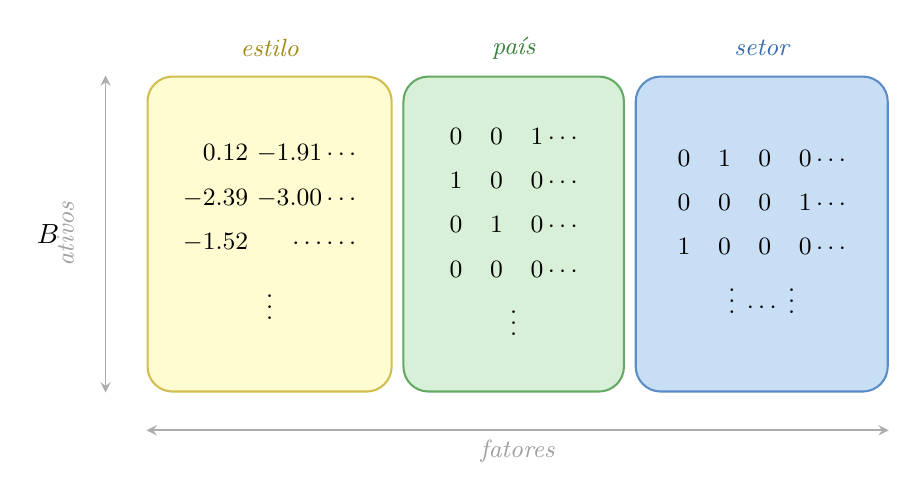
\begin{tikzpicture}[font=\small]

\definecolor{StyleFill}{RGB}{255,252,210}
\definecolor{StyleBorder}{RGB}{210,190,80}
\definecolor{StyleText}{RGB}{160,138,20}
\definecolor{CountryFill}{RGB}{215,240,215}
\definecolor{CountryBorder}{RGB}{100,170,100}
\definecolor{CountryText}{RGB}{60,130,60}
\definecolor{SectorFill}{RGB}{200,222,245}
\definecolor{SectorBorder}{RGB}{90,140,200}
\definecolor{SectorText}{RGB}{55,105,175}

% ── Bloco Estilo (x=0, w=3.1cm) ─────────────────────────────
\node[
    draw=StyleBorder, fill=StyleFill,
    rounded corners=9pt, line width=0.75pt,
    minimum width=3.1cm, minimum height=4.0cm,
    anchor=north west
] (style) at (0,0) {%
    $\begin{array}{r@{~}r@{~}l}
         0.12 & -1.91 & \!\cdots \\[5pt]
        -2.39 & -3.00 & \!\cdots \\[5pt]
        -1.52 & \cdots & \!\cdots \\[7pt]
        \multicolumn{3}{c}{\vdots}
    \end{array}$
};

% ── Bloco País (x=3.25cm, w=2.8cm) ──────────────────────────
\node[
    draw=CountryBorder, fill=CountryFill,
    rounded corners=9pt, line width=0.75pt,
    minimum width=2.8cm, minimum height=4.0cm,
    anchor=north west
] (country) at (3.25cm, 0) {%
    $\begin{array}{ccc@{~}l}
        0 & 0 & 1 & \!\cdots \\[5pt]
        1 & 0 & 0 & \!\cdots \\[5pt]
        0 & 1 & 0 & \!\cdots \\[5pt]
        0 & 0 & 0 & \!\cdots \\[3pt]
        \multicolumn{4}{c}{\vdots}
    \end{array}$
};

% ── Bloco Setor (x=6.2cm, w=3.1cm) ──────────────────────────
\node[
    draw=SectorBorder, fill=SectorFill,
    rounded corners=9pt, line width=0.75pt,
    minimum width=3.2cm, minimum height=4.0cm,
    anchor=north west
] (sector) at (6.2cm, 0) {%
    $\begin{array}{cccc@{~}l}
        0 & 1 & 0 & 0 & \!\cdots \\[5pt]
        0 & 0 & 0 & 1 & \!\cdots \\[5pt]
        1 & 0 & 0 & 0 & \!\cdots \\[3pt]
        \multicolumn{5}{c}{\vdots \;\cdots\; \vdots}
    \end{array}$
};

% ── Cabeçalhos em itálico colorido acima de cada bloco ──────
\node[StyleText,   font=\small\itshape] at ([yshift=0.35cm]style.north)   {estilo};
\node[CountryText, font=\small\itshape] at ([yshift=0.35cm]country.north) {pa\'{i}s};
\node[SectorText,  font=\small\itshape] at ([yshift=0.35cm]sector.north)  {setor};

% ── Seta horizontal "fatores" ────────────────────────────────
\draw[<->, >=stealth, line width=0.65pt, gray!65]
    ([yshift=-0.48cm]style.south west)
    -- node[below, font=\small\itshape, gray!75]{fatores}
    ([yshift=-0.48cm]sector.south east);

% ── Seta vertical + label "B  ativos" ───────────────────────
\draw[<->, >=stealth, line width=0.65pt, gray!65]
    ([xshift=-0.52cm]style.north west)
    --
    ([xshift=-0.52cm]style.south west);

% "ativos" rotacionado ao lado da seta
\node[font=\small\itshape, gray!75, rotate=90, anchor=south]
    at ([xshift=-0.80cm]style.west) {ativos};

% "B" à esquerda da seta
\node[font=\normalsize] at ([xshift=-1.25cm]style.west) {$B$};

\end{tikzpicture}
\caption{Estrutura típica da matriz de exposições fatoriais $B$,
particionada em blocos de estilo, pa\'{i}s e setor. As exposições de
estilo são valores contínuos padronizados; as exposições de pa\'{i}s e
setor são binárias, assumindo valor~1 se o ativo pertence àquela
categoria e 0 caso contrário \parencite{paleologo2025}.}
\label{fig:loadings_matrix}
\end{figure}
 
Nos modelos estatísticos, os fatores não são definidos a priori: tanto $B$ quanto $f_t$ são extraídos diretamente dos retornos observados por análise de componentes principais ou métodos correlatos. A lógica é que os padrões de co-movimento nos dados revelam as fontes latentes de risco sem que o pesquisador precise especificá-las antecipadamente. O PCA identifica as direções de máxima variância no painel de retornos e as usa como fatores, o que garante que os componentes extraídos explicam a maior parcela possível da variância total com o menor número possível de fatores. A desvantagem é que esses componentes não têm interpretação econômica direta: o primeiro fator estatístico tipicamente se assemelha ao portfólio de mercado, mas os demais são combinações lineares abstratas dos retornos sem correspondência imediata a variáveis observáveis.
 
A Análise de Componentes Principais Probabilística (PPCA), formalizada por \textcite{tipping1999}, oferece uma versão generativa dessa abordagem ao tratar os fatores como variáveis latentes com distribuição \textit{prior} Gaussiana. Nessa formulação, os retornos observados são realizações de um processo gerado pelos fatores latentes, e o problema de estimação consiste em inferir quais valores dos fatores são consistentes com os dados. Sob hipóteses Gaussianas, esse problema tem solução analítica: pela propriedade de conjugação Normal-Normal, o \textit{posterior} dos fatores dado os retornos observados é também Gaussiano, com média e covariância obtidas em forma fechada sem recorrer a métodos numéricos. Essa tratabilidade analítica é a razão pela qual o PPCA é adotado como modelo de referência neste trabalho. Ele representa o caso mais parcimonioso de um modelo fatorial probabilístico com \textit{posterior} analítico, e a comparação com ele isola precisamente o efeito da complexidade adicional do \textit{NeuralFactors} sobre as métricas de avaliação.
 
Nos modelos macroeconômicos, por fim, os fatores são séries observáveis como spreads de crédito, variações na taxa de inflação ou crescimento da produção industrial. As exposições são estimadas por regressão dos retornos individuais sobre essas séries em janelas temporais. Essa abordagem ancora os fatores em variáveis com interpretação econômica clara e permite estudar diretamente a transmissão de choques macroeconômicos ao mercado acionário, mas depende da escolha prévia das variáveis relevantes — e a teoria não oferece critério definitivo para essa seleção.
 
Apesar das diferenças entre as três abordagens, elas compartilham um conjunto de hipóteses que limitam sua capacidade de representar mercados com dinâmica de risco variável. Essas hipóteses não são falhas de implementação — são consequências estruturais da formulação linear estática, e compreendê-las é necessário para entender o que o \textit{NeuralFactors} se propõe a corrigir.
 
A primeira limitação é a estacionariedade das exposições. Em qualquer das três abordagens, a matriz $B$ é estimada sobre uma janela histórica de dados e mantida fixa ao longo do período de previsão. A sensibilidade de uma empresa ao câmbio, ao ciclo de commodities ou a um fator de estilo é tratada como constante, como se a estrutura de risco do ativo não variasse com o ambiente macroeconômico. Na prática, essa hipótese não se sustenta: empresas alteram sua estrutura de capital, mudam de segmento de atuação e redefinem sua exposição a fatores externos ao longo do tempo, e o próprio regime macroeconômico determina quais fontes de risco são dominantes em cada período. Um modelo estimado em um período de baixa volatilidade carregará exposições que podem subestimar sistematicamente o risco em períodos de estresse, exatamente quando estimativas precisas são mais necessárias para a gestão de carteiras.
 
A segunda limitação é a linearidade na extração dos fatores. Mesmo os modelos estatísticos, que não impõem estrutura econômica aos fatores, os extraem por métodos lineares como PCA. Isso significa que a estrutura de dependência entre ativos que o modelo captura é necessariamente linear e simétrica: a correlação entre dois ativos é tratada como constante ao longo do tempo, quando na prática as correlações entre ativos tendem a aumentar de forma pronunciada em momentos de crise. Esse fenômeno — correlações que se elevam precisamente quando a diversificação seria mais valiosa — é uma característica conhecida dos mercados financeiros que modelos lineares estáticos são estruturalmente incapazes de capturar. Relações não lineares entre características das empresas e seus retornos, ou padrões de dependência que emergem apenas sob condições extremas, ficam fora do alcance dessa classe de modelos.
 
A terceira limitação é distribucional. O modelo linear padrão com hipóteses Gaussianas produz uma distribuição conjunta dos retornos com caudas que decaem exponencialmente. Retornos financeiros, no entanto, apresentam caudas empiricamente mais pesadas: eventos que uma distribuição normal atribuiria probabilidade desprezível — quedas de três ou quatro desvios padrões em um único dia — ocorrem com frequência observável nos dados históricos. Para aplicações de gestão de risco como a calibração de \textit{Value at Risk}, essa discrepância tem consequências diretas: um modelo Gaussiano bem ajustado às condições normais de mercado subestimará sistematicamente as probabilidades de perdas extremas, produzindo estimativas de risco que falham precisamente nos cenários de estresse para os quais a modelagem existe.
 
Essas três limitações não são independentes entre si. Todas refletem uma mesma escolha subjacente: tratar o problema de estimação fatorial como estático, linear e Gaussiano. É precisamente essa escolha que o \textit{NeuralFactors} revisita, e as extensões que ele propõe respondem diretamente a cada uma dessas restrições.

\section{Modelos Fatoriais Probabilísticos}

A seção anterior encerrou com a observação de que os modelos fatoriais lineares clássicos compartilham uma limitação estrutural: os fatores são tratados como quantidades determinísticas, seja porque são definidos a priori (Fama-French, BARRA), seja porque são extraídos por técnicas de redução de dimensionalidade que não modelam incerteza (PCA). Os três problemas identificados (exposições estáticas, linearidade na extração dos fatores e hipótese Gaussiana) têm uma raiz comum nesse tratamento determinístico. Para resolver esse problema, é necessário um arcabouço que permita tratar os fatores como variáveis aleatórias não observadas, definir crenças sobre eles antes de ver os dados, e atualizar essas crenças de maneira coerente à medida que os retornos são observados. Esse arcabouço é a inferência bayesiana.

\subsection{Inferência Bayesiana e Variáveis Latentes}

A inferência bayesiana oferece uma linguagem formal para raciocinar sobre quantidades que não são diretamente observadas. No contexto de modelos fatoriais, os fatores de mercado, entendidos como as forças comuns que movem os retornos das ações de forma correlacionada, são precisamente esse tipo de quantidade. Em um dado dia de negociação, observa-se o vetor de retornos $r \in \mathbb{R}^N$ de $N$ ações, mas não se observa o vetor de fatores $z \in \mathbb{R}^F$ que supostamente gerou esses retornos. O fator $z$ é uma variável latente.

O raciocínio bayesiano sobre variáveis latentes se estrutura em três componentes. O *prior* $p(z)$ codifica a crença sobre os fatores antes de qualquer observação do dia; no caso de modelos fatoriais financeiros, o prior tipicamente expressa que os fatores têm média próxima de zero e dispersão compatível com a escala de retornos diários. A *verossimilhança* $p(r \mid z)$ especifica como os retornos observados se relacionam com os fatores latentes. Em um modelo fatorial linear, essa relação assume a forma $r = \alpha + Bz + \varepsilon$, onde $B$ é a matriz de exposições fatoriais e $\varepsilon$ captura o ruído idiossincrático de cada ação. O *posterior* $p(z \mid r)$ representa a crença atualizada sobre os fatores depois de observar os retornos. O teorema de Bayes conecta os três:

$$p(z \mid r) = \frac{p(r \mid z) \cdot p(z)}{p(r)}$$

onde $p(r) = \int p(r \mid z) \, p(z) \, dz$ é a verossimilhança marginal, obtida integrando sobre todos os valores possíveis dos fatores.

O posterior $p(z \mid r)$ é o objeto central da inferência bayesiana. Ele responde à pergunta: "dado que eu observei esses retornos hoje, qual é a distribuição de probabilidade sobre os fatores que provavelmente os geraram?" A resposta não é um único número, mas uma distribuição completa, que reflete a incerteza residual sobre os fatores mesmo após a observação dos dados. Quando se tem muitas ações informativas ($N$ grande) com exposições fatoriais altas e ruído idiossincrático baixo, o posterior se concentra em torno de um valor, pois há pouca dúvida sobre o que os fatores fizeram. Quando se tem poucas ações ou muito ruído, o posterior permanece disperso, sinalizando que os dados não são suficientes para determinar $z$ com precisão.

A distinção conceitual entre o tratamento determinístico e o bayesiano pode ser resumida da seguinte forma. No PCA clássico, a estimação dos fatores produz um ponto no espaço $\mathbb{R}^F$, a melhor estimativa de $z$, e descarta a informação sobre quão confiável essa estimativa é. Na abordagem bayesiana, a estimação produz uma distribuição sobre $\mathbb{R}^F$, preservando a incerteza. Essa incerteza é propagada para todas as quantidades derivadas: a covariância estimada entre os retornos, as previsões de risco, os portfólios ótimos. Por essa razão, modelos probabilísticos tendem a produzir estimativas de risco mais bem calibradas do que seus análogos determinísticos, já que a calibração depende diretamente de quantificar corretamente a incerteza, e não apenas de acertar a média.

Um resultado técnico que viabiliza a aplicação prática desse arcabouço a modelos fatoriais é a propriedade de *conjugação* da distribuição Gaussiana. Quando tanto o prior $p(z)$ quanto a verossimilhança $p(r \mid z)$ são Gaussianos, o posterior $p(z \mid r)$ também é Gaussiano e possui fórmula fechada, ou seja, a média e a covariância do posterior podem ser calculadas diretamente por operações matriciais, sem necessidade de aproximações numéricas ou algoritmos iterativos. Esse resultado é a base da regressão linear bayesiana e é o que permite que modelos fatoriais probabilísticos sejam computacionalmente tratáveis mesmo para centenas de ações.

A verossimilhança marginal $p(r)$ também desempenha um papel central nesse arcabouço. Essa quantidade mede a probabilidade dos retornos observados sob o modelo como um todo, integrando sobre todos os cenários possíveis de fatores ponderados por suas probabilidades a priori. Maximizar $p(r)$, ou equivalentemente minimizar a log-verossimilhança negativa, é o critério de treinamento natural para modelos generativos latentes. Em modelos lineares-Gaussianos, essa integral tem solução analítica. Em modelos mais complexos, onde a integral se torna intratável, a inferência variacional oferece uma alternativa: constrói-se um limite inferior, o \textit{Evidence Lower Bound} (ELBO), e otimiza-se esse limite. Essa ideia é o fundamento dos \textit{variational autoencoders} (VAEs), que serão discutidos na seção 2.2.3.


\subsection{Probabilistic PCA - Modelo Fatorial Generativo}

O PPCA (\textit{Probabilistic Principal Component Analysis}), proposto por Tipping e Bishop (1999) e por Roweis (1997) de forma independente, é a aplicação canônica do arcabouço bayesiano a modelos fatoriais. Ele reformula o PCA clássico, uma técnica de redução de dimensionalidade puramente algébrica, como um modelo generativo probabilístico com variáveis latentes.

O modelo generativo do PPCA assume que cada observação $x_i \in \mathbb{R}^d$ é gerada pelo seguinte processo:

$$z_i \sim \mathcal{N}(0, I_p)$$
$$x_i = \Lambda z_i + \mu + \varepsilon_i, \quad \varepsilon_i \sim \mathcal{N}(0, \sigma^2 I_d)$$

onde $z_i \in \mathbb{R}^p$ é o vetor de fatores latentes, $\Lambda \in \mathbb{R}^{d \times p}$ é a matriz de projeção (equivalente à matriz de exposições fatoriais $B$ na terminologia de modelos de precificação), $\mu$ é a média dos dados, e $\sigma^2$ é a variância do ruído, assumida igual em todas as dimensões (hipótese de ruído isotrópico).

Traduzindo para a linguagem de modelos fatoriais de equities: $x_i$ é o vetor de retornos de $d$ ações em um dado dia, $z_i$ é o vetor de $p$ fatores latentes que dirigem os co-movimentos entre as ações, $\Lambda$ é a matriz que mapeia fatores em retornos (as exposições fatoriais), e $\sigma^2$ captura a parte do retorno de cada ação que não é explicada pelos fatores comuns.

A distribuição marginal dos dados sob o PPCA é Gaussiana:

$$p(x_i) = \mathcal{N}(\mu, \Lambda\Lambda^\top + \sigma^2 I)$$

e a covariância implícita pelo modelo decompõe-se em dois termos: $\Lambda\Lambda^\top$, que captura a estrutura de correlação induzida pelos fatores comuns, e $\sigma^2 I$, que captura o ruído idiossincrático. Essa decomposição é formalmente idêntica à dos modelos fatoriais clássicos discutidos na seção 2.1; a diferença está no enquadramento probabilístico, que permite derivar tanto a distribuição dos dados quanto o posterior sobre os fatores.

O posterior sobre $z_i$ dado $x_i$ tem solução analítica, pela conjugação Normal-Normal:

$$p(z_i \mid x_i) = \mathcal{N}\left(\Lambda^\top(\Lambda\Lambda^\top + \sigma^2 I)^{-1}(x_i - \mu),\ I - \Lambda^\top(\Lambda\Lambda^\top + \sigma^2 I)^{-1}\Lambda\right)$$

Essa expressão tem a mesma estrutura da atualização bayesiana descrita na seção anterior: a média do posterior é uma combinação ponderada entre o prior (que puxa $z$ para zero) e a evidência dos dados (que puxa $z$ na direção que melhor explica os retornos observados), e a covariância do posterior é sempre menor que a do prior, refletindo a redução de incerteza proporcionada pela observação.

Os parâmetros $\Lambda$ e $\sigma^2$ podem ser estimados por máxima verossimilhança, e o PPCA possui uma propriedade notável: a solução de máxima verossimilhança para $\Lambda$ é diretamente relacionada aos autovetores da matriz de covariância amostral dos dados. Especificamente, as colunas de $\Lambda$ são os $p$ autovetores principais escalados pelas raízes dos autovalores correspondentes menos $\sigma^2$. Isso estabelece uma correspondência formal entre PCA (que extrai os autovetores dominantes) e PPCA (que os reinterpreta como parâmetros de um modelo generativo). Quando o ruído $\sigma^2$ tende a zero, o PPCA colapsa para o PCA determinístico: os fatores se tornam determinísticos e a incerteza desaparece.

Como modelo fatorial aplicado a ações, o PPCA resolve o problema central identificado nos modelos clássicos: os fatores passam a ser variáveis aleatórias com distribuição de probabilidade, e todo o aparato bayesiano (posterior, verossimilhança marginal, propagação de incerteza) fica disponível. O artigo NeuralFactors (Gopal, 2024) utiliza o PPCA como \textit{benchmark} comparativo, e reporta que embora o PPCA tenha desempenho inferior ao NeuralFactors em log-verossimilhança, ele produz estimativas de covariância e portfólios competitivos, justamente porque a estrutura probabilística garante coerência na quantificação de risco.

Entretanto, o PPCA herda limitações relevantes para a modelagem de retornos de ações. As exposições fatoriais $\Lambda$ são estimadas como parâmetros fixos, que não variam ao longo do tempo. Uma ação que muda de setor, que passa por uma reestruturação, ou cujo perfil de risco se altera com as condições macroeconômicas terá a mesma exposição fatorial durante todo o período de estimação. Além disso, os fatores latentes são extraídos exclusivamente a partir dos retornos passados. Informações fundamentalistas (múltiplos de \textit{valuation}, indicadores contábeis), indicadores de mercado (volatilidade implícita, \textit{spreads} de crédito) e classificações setoriais não entram na estimação, de modo que o modelo não tem como condicionar os parâmetros em fontes de informação externas aos retornos. Por fim, tanto o prior sobre $z$ quanto a verossimilhança são Gaussianos, o que implica que os retornos modelados seguem uma distribuição Gaussiana multivariada. Retornos de ações apresentam caudas pesadas, assimetria e agrupamento de volatilidade, fenômenos que a distribuição Gaussiana não captura adequadamente e que afetam diretamente a calibração de métricas de risco extremo como o \textit{Value at Risk}.


\subsection{NeuralFactors: Extensão Neural do Modelo Fatorial Probabilístico}

O NeuralFactors (Gopal, 2024) parte da estrutura fatorial probabilística do PPCA e a estende em três direções, cada uma voltada a uma das limitações remanescentes identificadas na seção anterior.

A extensão mais visível é tornar as exposições fatoriais variantes no tempo e condicionais em informação externa. No PPCA, a matriz $\Lambda$ é fixa; no NeuralFactors, os parâmetros por ativo (o intercepto $\alpha_{i,t}$, o vetor de exposições $\beta_{i,t}$, a escala idiossincrática $\sigma_{i,t}$ e os graus de liberdade $\nu_{i,t}$) são todos \textit{outputs} de uma rede neural chamada \textit{Stock Embedder}. Essa rede recebe como \textit{input} uma janela de $L=256$ dias úteis de \textit{features} temporais (retornos passados, indicadores fundamentalistas, índices de mercado) e \textit{features} estáticas (classificação setorial), e produz os quatro parâmetros para cada ação em cada data. Como consequência, as exposições fatoriais de uma ação se ajustam ao longo do tempo em resposta a mudanças nos seus fundamentos e no ambiente de mercado, sem que o analista precise redefinir manualmente os fatores ou reestimar o modelo periodicamente.

A arquitetura do Stock Embedder combina uma projeção linear por timestep, um Transformer Encoder de duas camadas que processa a sequência temporal, uma concatenação com as features estáticas, e um MLP de duas camadas que culmina em quatro cabeças lineares independentes para cada parâmetro. A escolha do Transformer como modelo de sequência reflete sua capacidade de capturar dependências de longo prazo na janela de lookback sem os problemas de gradiente que afetam LSTMs em sequências longas; o artigo demonstra empiricamente que a atenção supera o LSTM nessa aplicação.

O modelo também substitui a distribuição Gaussiana pela distribuição Student-T. No modelo generativo do NeuralFactors, o retorno de cada ação dado os fatores segue:

$$r_{i,t+1} \sim t_{\nu_{i,t}}(\alpha_{i,t} + \beta_{i,t}^\top z_{t+1},\ \sigma_{i,t})$$

onde $t_\nu$ denota a distribuição Student-T com $\nu$ graus de liberdade. A Student-T acomoda caudas mais pesadas que a Gaussiana: quando $\nu$ é pequeno, eventos extremos recebem probabilidade substancialmente maior do que sob a normal. Os graus de liberdade $\nu_{i,t}$ são aprendidos por ação e por data, o que permite ao modelo calibrar a frequência de eventos extremos de forma granular. Da mesma forma, o prior sobre os fatores latentes também é Student-T:

$$z_{t+1} \sim t_{\nu_z}(\mu_z, \sigma_z)$$

com parâmetros $\mu_z$, $\sigma_z$ e $\nu_z$ aprendidos durante o treinamento. Essa escolha distribucional tem consequências diretas para a calibração de métricas de risco: a distribuição Student-T permite que os quantis extremos, ou seja, os percentis que definem o \textit{Value at Risk}, sejam mais conservadores do que os previstos por um modelo Gaussiano, refletindo a frequência real de perdas extremas em mercados de ações.

Por fim, a introdução da Student-T torna a integral da verossimilhança marginal $p(r) = \int p(r \mid z) p(z) dz$ intratável, pois o produto de uma verossimilhança Student-T com um prior Student-T não possui posterior em forma fechada. O NeuralFactors contorna essa dificuldade combinando duas técnicas. Primeiro, aplica \textit{moment matching} para aproximar a Student-T do prior por uma Gaussiana com mesmos dois primeiros momentos, o que permite calcular o posterior $q(z \mid r)$ em forma fechada via regressão linear bayesiana, da mesma forma que no PPCA. Segundo, para compensar o erro de aproximação introduzido pelo *moment matching*, utiliza o \textit{Importance Weighted Autoencoder} (IWAE) como objetivo de treinamento em vez do ELBO padrão. O IWAE, proposto por Burda et al. (2016), gera $K$ amostras do posterior aproximado e pondera cada uma por sua razão de importância $p(r \mid z^{(k)}) p(z^{(k)}) / q(z^{(k)} \mid r)$, resultando em um estimador com menor viés que o ELBO. O artigo utiliza $K=20$ amostras e a versão condicional da \textit{loss}, o CIWAE (\textit{Conditional IWAE}), que condiciona toda a computação na informação histórica $\mathcal{F}_t$.

A arquitetura resultante pode ser interpretada como uma cadeia de três blocos funcionais. O Stock Embedder transforma \textit{features} em parâmetros do modelo fatorial por ativo. O encoder combina esses parâmetros com os retornos observados para computar o posterior sobre os fatores via regressão linear bayesiana, uma operação puramente algébrica sem pesos neurais próprios. O decoder avalia a verossimilhança dos retornos observados dado cada amostra dos fatores. A \textit{loss} CIWAE combina as contribuições dos três blocos e seus gradientes fluem de volta ao \textit{Stock Embedder} (que concentra todos os parâmetros treináveis da rede) e aos parâmetros do prior.

Uma propriedade relevante para aplicações práticas é que a média e a covariância dos retornos sob o modelo podem ser calculadas em forma fechada, sem amostragem:

$$\mathbb{E}[r] = \alpha + B^\top \mu_z, \quad \text{Cov}(r) = \Sigma_x + B^\top \Sigma_z B$$

onde $\Sigma_x = \text{diag}(\sigma_1^2, \ldots, \sigma_N^2)$ é a covariância idiossincrática e $B$ é a matriz de exposições. Essa propriedade permite que o modelo seja utilizado diretamente para otimização de portfólios de mínima variância e para estimação de risco, sem a necessidade de simulação de Monte Carlo para obter a covariância. Trata-se de uma vantagem computacional sobre modelos generativos puramente neurais que não possuem estrutura fatorial.

O NeuralFactors herda portanto a interpretabilidade dos modelos fatoriais clássicos (decomposição de retornos em componentes sistemáticos e idiossincráticos, exposições fatoriais por ativo) e a coerência probabilística do PPCA (posterior sobre fatores, propagação de incerteza, treinamento por máxima verossimilhança), ao mesmo tempo em que relaxa as restrições de exposições estáticas, features limitadas a retornos, e distribuição Gaussiana que limitavam esses modelos predecessores.